\chapter{Formal analogical proportions}
\label{CHAP:formal_analogical_proportions}
\localtableofcontents*
\vspace*{\baselineskip}

\initial{A}fter a first introduction of past works on analogical reasoning in
Chapter \ref{CHAP:computational_models_of_analogical_reasoning}, we will now
provide all the necessary background on formal analogical proportions, the most
important concept of this document.

An \textbf{analogical proportion} is a statement of the form ``$a$ is to $b$ as
$c$ is to $d$''. It is a relation between the two pairs $(a,b)$ and $(c,d)$,
which expresses that what is common to $a$ and $b$ is also common to $c$ and
$d$, and what is different between $a$ and $b$ is also different between $c$
and $d$. There are numerous examples of such statements, with which everybody
will more or less agree, such as  ``a calf is to a cow as a foal is to a
mare'', or ``Paris is to France as Berlin is to Germany''.  As a relation
involving both similarities \textbf{and} dissimilarities between four objects,
an analogical proportion is able to model complex associations.

\paragraph{The three axioms of analogical proportions\\}

It has been agreed since Aristotle time that an analogical proportion $A$ is a
quaternary relation satisfying the \textbf{three following axioms}, for any $a,
b, c, d$:

\begin{enumerate}
\item $A(a,b,a,b)$ always holds (Reflexivity)
\item $A(a,b,c,d) \implies A(c,d,a,b)$ (Symmetry)
\item $A(a,b,c,d) \implies A(a,c,b,d)$ (Central permutation)
\end{enumerate}

When there is no ambiguity over $A$ and its domain, the infix notation
$a:b::c:d$ is often used. Considering again the farm example, the symmetry
axiom states that if a calf $(a)$ is to a cow $(b)$ as a foal $(c)$ is to a
mare $(d)$, then a foal $(c)$ is to a mare $(d)$ as a calf $(a)$ is to a cow
$(b)$, which seems perfectly sound. The central permutation axiom leads to the
natural consequence that a calf $(a)$ is to a foal $(c)$ as a cow $(b)$ is to a
mare $(d)$.

This chapter is structured as follows. In the first section of this chapter, we
will provide the definition of analogical proportions in various settings, with
a strong emphasis on the arithmetic and Boolean proportions, which will turn
out to be very close. We will further investigate this bond in the second
section, which will be devoted to describe these two proportions from a
geometrical perspective. In the last section, we will consider a toy
classification problem, which will help us introduce two other key concepts:
the \textbf{analogical inference principle}, and the process of
\textbf{analogical equation solving}. This last section will also serve as a
transition towards the next chapter, which will be devoted to describe our
contributions to analogical classification.

\section{Formal definitions}
\label{SEC:formal_definitions_proportions}

The goal of this first section is to provide the definitions of analogical
proportions in various settings. We will particularly focus on the arithmetic
proportion that deals with real numbers, and on the Boolean proportion.

\subsection{The geometric and arithmetic proportions}

\paragraph{A factorization-based definition of analogical proportions\\}

Probably the first use of formal proportions is that of Lepage in \cite{Lep04}
who, starting from the three aforementioned axioms, formally defined analogical
proportions over alphabets of letters with the aim of generating (analogical)
formal languages. His definition have later been generalized in the works of
Stroppa and Yvon (see \cite{StrYvoCNLL05} and \cite{StrYvoREPORT05}), who
provided an algebraic factorization-based definition of analogical proportions
in semigroups:

\begin{definition}[Proportion in semigroups]
\label{DEF:proportion_semi_group}
Let $(U, \oplus)$ be a semigroup, i.e. $U$ is a set and $\oplus$ is an
  associative binary operation. Four elements $a, b, c, d \in U$, are in proportion if
  there exists some factorization
  \begin{align*}
    a &= a_1 \oplus a_2 \oplus \cdots \oplus a_n\\
    b &= b_1 \oplus b_2 \oplus \cdots \oplus b_n\\
    c &= c_1 \oplus c_2 \oplus \cdots \oplus c_n\\
    d &= d_1 \oplus d_2 \oplus \cdots \oplus d_n,
  \end{align*}

  such that for all $i \in [1, n]$,
  $$
  \begin{cases}
    a_i = b_i \text{ and } c_i = d_i\\
    \text{or}\\
    a_i = c_i \text{ and } b_i = d_i.
  \end{cases}
  $$
\end{definition}

\begin{testexample}
  A use of this definition can be found in \cite{StrYvoREPORT05}, where
  the authors define an analogy between words of a finite alphabet using the
  concatenation operator, which allows to build proportions such as:
  $$\text{eat} : \text{eating} :: \text{look} : \text{looking}.$$ This analogy
  was used in an automatic verb conjugation task that we will briefly describe
  in the next chapter.
\end{testexample}

\paragraph{Analogical proportions between real numbers\\}

To further illustrate the use of Definition \ref{DEF:proportion_semi_group}, it
will be insightful to instantiate $U$ as the set of natural number $\mathbb{N}$
and $\oplus$ as the usual multiplication $\times$.
\begin{testexample}
  In this setting, let's consider the prime factorization of:

  \begin{align*}
    a &= 30 = 1 \times 2 \times 3 \times 5\\
    b &= 60 = 2 \times 2 \times 3 \times 5\\
    c &= 25 = 1 \times 1 \times 5 \times 5\\
    d &= 50 = 2 \times 1 \times 5 \times 5.
  \end{align*}

For each $i$, we either have $a_i = b_i$ and $c_i = d_i$ ($i = 2, 3, 4$) or
$a_i = c_i$ and $b_i = d_i$ ($i = 1, 4$). We can then say that $a, b, c, d$ are
in proportion, i.e. $30: 60 :: 25: 50$. We recognize here the \textbf{geometric
  proportion}: $\frac{30}{60} = \frac{25}{50}$.
\end{testexample}

\begin{definition}[Geometric proportion]
  Four elements $a, b, c, d$ in $\mathbb{R}$ are in \textbf{geometric
  proportion} if
  $$\frac{a}{b} = \frac{c}{d},$$
  or equivalently if
  $$a\times d = b\times c.$$
\end{definition}

It now becomes clear why analogical proportions are effectively called
\textit{proportions}: it is precisely because they generalize the well-known
numerical geometric proportion to more complex structures.  Actually, Aristotle
stated the three aforementioned axioms on the basis of the geometric
proportion.

In fact, when $\mathbb{R}$ is equipped with the multiplication $\times$, the
couple $(\mathbb{R}, \times)$ is a group (i.e. a set equipped with an operation
that satisfies  closure, associativity, identity and invertibility). When
dealing with a group (instead of a semigroup), Definition
\ref{DEF:proportion_semi_group} can be greatly simplified:

\begin{definition}[Proportion in groups]
  \label{DEF:proportion_group}
Let $(U, \oplus)$ be a group.  Four elements $a, b, c, d \in U$, are in
  proportion if:
  $$a \oplus d = b \oplus c.$$
\end{definition}

The geometric proportion is clearly a direct instance of this definition.
Another proportion can be defined over real numbers, using this time the
addition operator $+$ for the group $(\mathbb{R}, +)$:

\begin{definition}[Arithmetic proportion]
  Four elements $a, b, c, d$ in $\mathbb{R}$ are in \textbf{arithmetic
  proportion} if:
  $$a + d = b + c,$$
  or equivalently if
  $$a - b = c - d.$$
\end{definition}

\paragraph{Analogical proportions over vectors\\}

An analogical proportion in $\mathbb{R}$ is great, but what will be more useful
is a proportion in $\mathbb{R}^m$, so that we can deal with vectors.  Let us
make a brief notation note: in the rest of this document, vectors will be
denoted by boldface letters and their components will be denoted by regular
letters. For example, a vector $\mathbf{x} \in X^m$ will be defined as
$\mathbf{x} = (x_1, x_2, \dots, x_m)$.

It is actually fairly easy to define a proportion in a given set $X^m$ provided
that we already have a proportion in $X$. Indeed, a natural extension to $X^m$
is to require that each of the $m$ dimensions make up valid proportions in $X$:

\begin{definition}[Proportion for vectors]
  \label{DEF:analogy_for_vectors}
  Let $A$ be an analogy over a set $X$. We can define an analogy $A^m$ over
  $X^m$ in a component-wise fashion by:
  $$A^m(\mathbf{a}, \mathbf{b}, \mathbf{c}, \mathbf{d}) ~ \text{  if  } ~
  A(a_i, b_i, c_i, d_i) \text{ for all } i \in [1, m],$$
  where $\mathbf{a}, \mathbf{b}, \mathbf{c}, \mathbf{d}$ are vectors in $X^m$.
  More often than not, $A^m$ will simply be denoted $A$ for the sake of
  brevity.
\end{definition}
\noindent
Thanks to Definition \ref{DEF:analogy_for_vectors}, we now have the definition
of two numerical proportions in $\mathbb{R}^m$: one that generalizes the
geometric proportion and one that generalizes the arithmetic proportion.  The
interpretation of the geometric proportion in $\mathbb{R}^m$ can be opaque, but
that of the arithmetic proportion is very clear: four vectors $\mathbf{a},
\mathbf{b}, \mathbf{c}, \mathbf{d}$ of $\mathbb{R}^m$ are in arithmetic
proportion if $\mathbf{a} - \mathbf{b} = \mathbf{c} - \mathbf{d}$, i.e.
\textbf{if they are the four vertices of a parallelogram}, as illustrated in
Figure \ref{FIG:arithmetic_proportion}.
\begin{figure}[!h]
\centering
  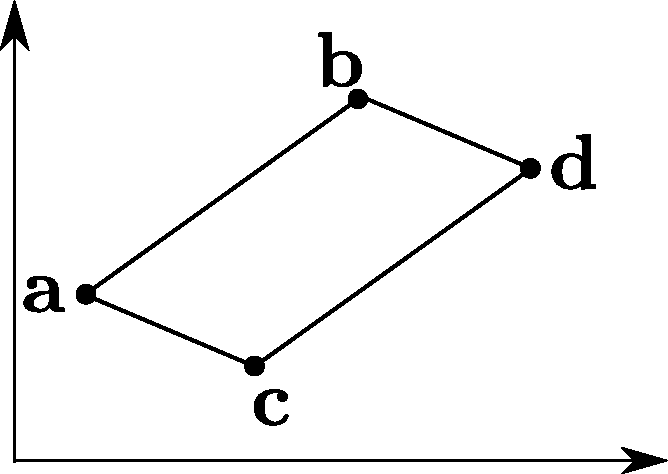
\includegraphics[width=2.5in]{figures/arithmetic_proportion.pdf}
  \caption{$\mathbf{a}, \mathbf{b}, \mathbf{c}, \mathbf{d}$
  are in arithmetic proportion iff they are the four vertices of a
  parallelogram.}
\label{FIG:arithmetic_proportion}
\end{figure}

Let us mention that even if they did not explicitly mention the parallelogram
view of analogy, Rumelhart and Abrahamsen (Section
\ref{SEC:rumelhart_Abrahamsen}) clearly used the arithmetic proportion for
their psychological model of analogical reasoning.

Starting from the general lines of Definition \ref{DEF:proportion_semi_group},
other proportions have been defined in various domains, e.g. analogies
between trees, lattices, or matrices \cite{MicDel04, StrYvoREPORT05,
MicBayDelJAIR08}. However, we will not detail them further here and rather
focus on other domains of interest, namely analogies between sets. Defining
analogies between sets will indeed allow us to derive the definition of an
analogical proportion for Boolean values, which is the main subject of this
document.

\subsection{Analogical proportions between sets}

In \cite{Lep03}, Lepage defines an analogy between sets as follows: four subsets
$A, B, C, D$ of a universal set $X$ are in proportion if $A$ can be transformed
into $B$ by adding and deleting the same elements as to transform $C$ into $D$.
A more formal definition has been given in \cite{StrYvoREPORT05}:

\begin{definition}[Proportion between sets (i)]
  \label{DEF:analogy_set_facto}
  Let $A, B, C, D \subset X$. $A, B, C, D$ are in proportion if there exists
  four subsets $U, V, W$ and $Z$ (not necessarily disjoint) such that:
  $$
  \begin{cases}
    A = U \cup V\\
    B = U \cup W\\
    C = Z \cup V\\
    D = Z \cup W.
  \end{cases}
  $$
\end{definition}

The requirements of Lepage are clearly respected here: to go from $A$ to $B$,
one needs to add $W$ and remove $V$. To go from $C$ to $D$, one needs to do the
exact same thing: add $W$ and remove $V$. This definition is completely
compliant with our informal introduction at the beginning of this chapter,
where we explained that an analogical proportion $a:b::c:d$ expresses that
\textit{what is common to $a$ and $b$ is also common to $c$ and $d$, and what
is different between $a$ and $b$ is also different between $c$ and $d$}.


An equivalent definition of analogy between sets has been given in
\cite{MicPra09}:

\begin{definition}[Proportion between sets (ii)]
  \label{DEF:analogy_set_miclet_henri}
  Let $A, B, C, D \subset X$. $A, B, C, D$ are in proportion if:
  $$
  A \setminus B = C \setminus D \text{ and } B \setminus A = D \setminus C.
  $$
\end{definition}

Definition \ref{DEF:analogy_set_miclet_henri} reads as \textit{$A$ differs from
$B$ as $C$ differs from $D$, and $B$ differs from $A$ as $D$ differs from $C$},
which is naturally equivalent to the statement of Definition
\ref{DEF:analogy_set_facto}: $A \setminus B = C \setminus D = V$, and $B
\setminus A = D \setminus A  = W$.  Finally, a last equivalent definition can
be given as follows (not without using various ingenious tweaks):

\begin{definition}[Proportion between sets (iii)]
  \label{DEF:yet_other_equiv_def}
  Let $A, B, C, D \subset X$. $A, B, C, D$ are in proportion if:
  $$ A \cap D = B \cap C \text{ and } A \cup D = B \cup C.$$
\end{definition}

\noindent
These three equivalent definitions are illustrated in Figure
\ref{FIG:equiv_analogies_sets}.

\begin{figure}[!h]
\centering
  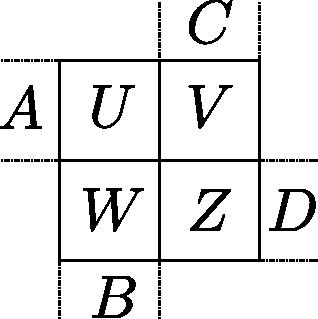
\includegraphics[width=1in]{figures/subset_analogies.pdf}
  \caption{The four sets $A, B, C, D$ are in proportion. In general, $U, V,W,
  Z$ do not need to be disjoint.}
\label{FIG:equiv_analogies_sets}
\end{figure}

\begin{testexample}
For a more concrete example, let us consider $A = \{a, b, c, g\}, B = \{a, b,
d, e, g\}, C = \{c, f, g\}$ and $D = \{d, e, f, g\}$, as summed-up in Table
\ref{TAB:analogy_sets}.
Setting $U = \{a, b, g\}, V = \{c\}, W = \{d, e\}$ and $Z = \{f, g\}$, the
conditions of Definition  \ref{DEF:analogy_set_facto}  are clearly satisfied.
Also, $A \setminus B = C \setminus D = \{c\} = V$, and $B\setminus A = D
\setminus C = \{d, e\} = W$. Finally, $A \cup D = B \cup C = \{a, b, c, d, e,
f, g\}$ and $A\cap D = B\cap C = \{g\}$.
\end{testexample}
\begin{table}[h!]
\centering
$$
\begin{tabular}{ c  c  c  c  c  c  c  c }
\toprule
  & a & b & c & d & e & f & g\\
\midrule
  A & \times & \times & \times &  &  &  & \times \\
  B & \times & \times &  & \times & \times &  & \times\\
  C &  &  & \times &  &  & \times & \times\\
  D &  &  &  & \times & \times & \times & \times\\
\bottomrule
\end{tabular}
$$
\caption{Four sets $A, B, C, D$ in analogical proportion.}
\label{TAB:analogy_sets}
\end{table}

Analogies between sets are important because they allow us to derive the
definition of the Boolean proportion, which is the object of the next
subsection.

\subsection{The Boolean proportion}

\paragraph{Formal definition\\}

We are now in a position to give a formal definition of the Boolean proportion,
which can be directly derived from Definitions
\ref{DEF:analogy_set_miclet_henri} or \ref{DEF:yet_other_equiv_def} by
considering the set $\mathbb{B} = \{0, 1\}$:

\begin{definition}[Boolean proportion (i)]
  \label{DEF:boolean_proportion}
  Four elements $a, b, c, d$ in $\mathbb{B} = \{0, 1\}$ are in \textbf{Boolean
  proportion} if
  \begin{align*}
    &\left[(a \wedge \neg b) \leftrightarrow (c \wedge \neg d)\right]  \wedge
    \left[(\neg a \wedge b)\leftrightarrow (\neg c \wedge d)\right], \text{ or equivalently}\\
    &  (a \wedge d \leftrightarrow b \wedge c) \wedge (a \vee  d
    \leftrightarrow b \vee c),
  \end{align*}
  where $\leftrightarrow$ stands for the equivalence connective.
\end{definition}

The first expression is the direct counterpart of Definition
\ref{DEF:analogy_set_miclet_henri}, and states that \textbf{$a$ differs from
$b$ as $c$ differs from $d$, and conversely $b$ differs from $a$ as $d$ differs
from $c$}.  The second expression directly comes from Definition
\ref{DEF:yet_other_equiv_def}.

In a Boolean setting, there are exactly $2^4 = 16$ different valuations of $a,
b, c, d$. Definition \ref{DEF:boolean_proportion} tells us that exactly $6$ of
these valuations (or \textbf{patterns}) lead to valid Boolean proportions.
Table \ref{TAB:six_valid_patterns} illustrates the $6$ valid patterns and the
$10$ invalid ones. We recognize in Table \ref{TAB:six_valid_patterns} that all
the valid patterns express that we need to perform the same operation to go
from $a$ to $b$ as to go from $c$ to $d$, and that this is not the case for the
invalid patterns. This is compliant with what we expect from an analogical
proportion, as discussed earlier. With regards to this, the last two invalid
patterns (namely $0:1::1:0$ and its counterpart $1:0:0:1$) have a particular
status: we could indeed claim that they express the fact that $b$ is the
negation of $a$ just like $c$ is the negation of $d$, so in some sense we
\textbf{still} could say that $a$ differs from $b$ as $c$ differs from $d$. We
will discuss this point further when we will mention the works of Sheldon
Klein, who came up with a different definition of the Boolean analogical
proportion.

\begin{table}[t]
  \centering
  \begin{tabular}[t]{ccccc}
    \toprule
    $a$ & $b$ & $c$ & $d$ &  $A(a, b, c, d)$\\
    \midrule
    0 & 0 & 0 & 0 &   \textbf{1}\\
    1 & 1 & 1 & 1 &   \textbf{1}\\
    0 & 0 & 1 & 1 &   \textbf{1}\\
    1 & 1 & 0 & 0 &   \textbf{1}\\
    0 & 1 & 0 & 1 &   \textbf{1}\\
    1 & 0 & 1 & 0 &   \textbf{1}\\
    \bottomrule
  \end{tabular}
  ~~~~
  \begin{tabular}[t]{ccccc}
    \toprule
    $a$ & $b$ & $c$ & $d$ &  $A(a, b, c, d)$\\
    \midrule
    0 & 0 & 0 & 1 &   \textbf{0}\\
    0 & 0 & 1 & 0 &   \textbf{0}\\
    0 & 1 & 0 & 0 &   \textbf{0}\\
    1 & 0 & 0 & 0 &   \textbf{0}\\
    1 & 1 & 1 & 0 &   \textbf{0}\\
    1 & 1 & 0 & 1 &   \textbf{0}\\
    1 & 0 & 1 & 1 &   \textbf{0}\\
    0 & 1 & 1 & 1 &   \textbf{0}\\
    0 & 1 & 1 & 0 &   \textbf{0}\\
    1 & 0 & 0 & 1 &   \textbf{0}\\
    \bottomrule
  \end{tabular}
  \caption{The six valid patterns of the Boolean proportion (left), and the ten
  invalid patterns (right).}
  \label{TAB:six_valid_patterns}
\end{table}

We observe from Table \ref{TAB:six_valid_patterns} that some
sort of {\it code independence axiom} is satisfied, which guarantees that $0$
and $1$ play symmetric roles:
\begin{property}
  \label{PROPER:code_indep}
  Let a, b, c, d in $\mathbb{B}$. Then
  $$a : b :: c : d \iff \neg a :  \neg b ::  \neg c :  \neg d,$$
  where $\neg x$ is the negation of $x$.
\end{property}
This code independence property is actually extremely important for
representational purposes, because it means that we do not have to care about
the coding convention of the Boolean vectors that we use.

We gave the definition of the Boolean proportion as a consequence of the
definition of proportions between sets, but let us note that in fact, the $6$
valid patterns of Table \ref{TAB:six_valid_patterns} could have been derived
directly from the $3$ axioms of an analogical proportion: the first axiom tells
us that the proportion $a:b::a:b$ holds for any value of $a$ and $b$ in
$\mathbb{B}$. This means that the four following proportions are valid:
\begin{itemize}
  \item $0 : 1 :: 0 :1$ ;
  \item $1 : 0 :: 1 :0$ ;
  \item $0 : 0 :: 0 :0$ ;
  \item $1 : 1 :: 1 :1$.
\end{itemize}
Using the central permutation axiom $(a:b::c:d \iff a:c::b:d$), we can then
derive two additional proportions, which makes a total of $6$ proportions that
are indeed those of Table \ref{TAB:six_valid_patterns}:
\begin{itemize}
  \item $1 : 1 :: 0 : 0$ ;
  \item $0 : 0 :: 1 : 1$.
\end{itemize}

\paragraph{The Boolean proportion as a particular case of the arithmetic
proportion\\}

By paying attention to Table \ref{TAB:six_valid_patterns}, we notice that the
Boolean proportion can actually be defined in a simpler way:
\begin{definition}[Boolean proportion (ii)]
  \label{DEF:boolean_proportion_informal}
  Four elements $a, b, c, d$ in $\mathbb{B}$ are in \textbf{Boolean proportion} if:
  $$
  \begin{cases}
    a = b \text{ and } c = d\\
    \text{or}\\
    a = c \text{ and } b = d,
  \end{cases}
  $$
  or equivalently if
  $$a - b = c - d.$$
\end{definition}

Naturally, the values $a - b$ and $c -d$ do not necessarily belong to
$\mathbb{B}$, but it does not really matter: we just have to temporarily
consider that $a, b, c, d$ are in $\mathbb{R}$. We are here witnessing a close
bond that links the Boolean proportion and the arithmetic proportion:
\textbf{when restricted to $\mathbb{B}$, the arithmetic proportion and the
Boolean proportion are equivalent}. The connections between these two
proportions will be more and more obvious as we go through this document.

If the Boolean and the arithmetic proportion are equivalent in $\mathbb{B}$, the
geometric proportion only offers a necessary condition to define the Boolean
proportion: $a \times d = b\times c$ is satisfied by all of the valid patterns
in Table \ref{TAB:six_valid_patterns}, but also for the pattern $0: 0: 0: 1$
which is not a valid analogy. In that sense, the Boolean proportion is closer
to the arithmetic proportion than to the geometric proportion.

\paragraph{The Boolean proportion of Sheldon Klein\\}

We cannot talk about formal Boolean proportions without going back to the 80s
and mention the pioneering work of Sheldon Klein who, to some extent, defined
his \textit{own} Boolean analogical proportion \cite{Kle83}. His definition
states that $a, b, c, d$ in $\mathbb{B}$ are in proportion if $a \oplus b = c
\oplus d$, where $\oplus$ is the XOR operator.  This definition is less
restrictive than Definition \ref{DEF:boolean_proportion}, and amounts to
considering that in addition to the $6$ valid patterns from Table
\ref{TAB:six_valid_patterns}, two other patterns are also valid, namely
$0:1::1:0$ and its counterpart $1:0::0:1$.

These two patterns seem appealing at first sight, because they capture the fact
that $a : \neg a :: b : \neg b$. However, they also lead to the fact that
$a:b::c:d \iff b : a :: c :d$, which seems quite unnatural for an analogy.
Indeed, if a calf $(a)$ is to a cow $(b)$ as a foal $(c)$ is to a horse $(d)$,
it seems unnatural to say that a cow $(b)$ is to a calf $(a)$ as a foal $(c)$
is to a horse $(d)$. This notion will become clear in the next section when we
will present the equivalence classes of analogical proportion (here, $(a, b, c,
d)$ and $(b, a, c, d)$ are not in the same equivalence class).  In practice, it
is often observed that using the modeling of Klein leads to less accurate
learners than using the standard modeling.

In fact, Klein's definition of the Boolean proportion $a:b::c:d \iff a
\oplus b = c \oplus d$ is equivalent to $a \oplus d = b \oplus c$, due to the
singular properties of the XOR operator. This definition is actually a direct
instance of Definition \ref{DEF:proportion_group} (analogies in groups), which
is natural because of the fact that when the set $B = \Set{0, 1}$ is equipped
with the XOR operator, we obtain a group.

\paragraph{The logical proportion of Jean Piaget and its generalization\\}
Another remarkable precursor work is that of Jean Piaget who, in the annex of a
French book from 1952 \cite{Pia52}, defined what he called a \textit{logical
proportion} as follows: four propositions $a, b, c,d$ are in proportion if $(a
\wedge d \leftrightarrow b \wedge c) \wedge (a \vee  d \leftrightarrow b \vee
c)$. This definition is clearly equivalent to what we refer to now as the
Boolean \textbf{analogical} proportion, and was likely derived by Piaget when
he was trying to give a Boolean counterpart to the geometric proportion, where
the exchange of extreme and means plays a key role. In fact, it turns out that
Piaget never made any reference to analogy in this work.

This concept of \textbf{logical proportion} has been generalized in recent
works (see e.g. \cite{PraRic13LU}). A logical proportion is here defined as a
couple of equivalences of the form:

$$I_1(a, b) \leftrightarrow I_2(c, d) ~~ \wedge ~~ I_3(a, b) \leftrightarrow I_4(c,
d),$$
where $a, b, c, d$ are Boolean variables and each $I_i$ is either an
\textbf{indicator of similarity} or an \textbf{indicator of dissimilarity}. An
indicator of similarity $I(x, y)$ is either of the form $x \wedge y$  or
of the form $\neg x \wedge \neg y$: it captures what is common to $x$ and $y$,
or what is both not in $x$ and not in $y$. Conversely, a dissimilarity indicator $I(x,
y)$ will be of the form $\neg x \wedge y$ or $x \wedge \neg y$,  and captures
what is in $y$ and not in $x$, or what is in $x$ and not in $y$.  A logical
proportion then expresses a semantic equivalence between the two pairs of
variables $(a, b)$ and $(c, d)$, in terms of similarities and/or
dissimilarities. The Boolean analogical proportion that we are studying here is
a particular instance of logical proportion.

There is a total $120$ possible logical proportions (see \cite{PraRic12} for a
derivation), and quite interestingly each of these logical proportions are
true for exactly $6$ valuations of $a, b, c, d$. This makes them quite rare,
because there are in fact $\binom{16}{6} = 8008$ propositions that are true for
$6$ valuations only, out of the $16$ possible valuations. Out of these $120$
logical proportions, only $8$ of them support the code independency property
(Property \ref{PROPER:code_indep}) which makes the remaining $112$ proportions
unsuitable for representational purposes.

Out of these $8$ code-independent proportions, $4$ proportions exhibit
interesting cognitive properties, that we name the \textbf{homogeneous}
proportions. These proportions are characterized by the fact that all the
expressions $I_i(x, y)$ are different, and by the fact that $I_1$ and $I_2$ are
of the same kind (i.e. they are both similarity indicators, or both
dissimilarity indicators), and the same goes for $I_3$ and $I_4$. These four
proportions are called the paralogy, the reverse analogy, the inverse paralogy,
and naturally the \textbf{analogy}. We will however not make use of these
logical proportions in this document (except the Boolean analogical proportion of
course!), so we will not detail them further.

\paragraph{Extension to multiple-valued logics\\}

In \cite{PraRic13}, the authors propose an extension of the Boolean proportion
to a multiple-valued logic where the elements can take real values in the
interval $[0, 1]$.  This extension was proposed on the basis of the definition
$A(a, b, c, d) \iff \left[(a \wedge \neg b) \leftrightarrow (c \wedge \neg
d)\right]  \wedge \left[(\neg a \wedge b)\leftrightarrow (\neg c \wedge
d)\right]$, and using the following mapping between operators:
\begin{itemize}
  \item The central $\wedge$ becomes to the min operator.
  \item $x \leftrightarrow y$ becomes $1 - |x - y|$.
  \item $x \wedge \neg y$ becomes $\max(0, x-y)$.
\end{itemize}
The graded view of the analogical proportion then becomes:
\begin{align*}
A(a, b, c, d) =
\begin{cases}
  1 - |(a - b) - (c - d)| &\text{ if } a \geq b \text { and } c \geq d, \text{
    or } a \leq b \text{ and } c \leq d\\
  1 - \max(|a - b|, |c - d|) &\text{ if } a \geq b \text { and } c \leq d, \text{
    or } a \leq b \text{ and } c \geq d.
\end{cases}
\end{align*}
The conditions may seem complicated but they actually express simple facts: the
first one states that $a$ differs from $b$ in the same direction as $c$ differs
from $d$, and the second one states the reverse. It is clear that this
definition is quite closely linked to that of the arithmetic proportion.

Let us note that there are other ways to transform the Boolean operators into
multiple-valued logic operators. If we had started from a different expression
of the Boolean proportion, or if we had used alternative choices of operators,
we would have ended up with a different potential definition of this analogical
proportion. However, some combinations lead to definitions that do not
completely suit the requirements that one can expect from an analogical
proportion. So in practice, the choice of operators is dictated by the
plausibility of the final expression (see \cite{PraRic13} for a discussion).
We here chose to describe this definition because of its links to the
arithmetic proportion, and because  we will make use of this graded view of
analogy later in Chapter \ref{CHAP:analogical_recommendation}.

\paragraph{Conclusion\\}
This first section was devoted to the description of various definitions of
analogical proportions in different settings: we have reviewed analogies between
real numbers, between sets, between Boolean numbers, and an extension to
multiple-valued logics. In this document, the two kinds of proportions that we
will deal with are the Boolean proportion and the arithmetic proportion, which
we have shown to be extremely close. As having a deep understanding of how
these two proportions work will be very insightful for us, the next section is
devoted to give a geometrical interpretation of the Boolean and arithmetic
proportions.

\section{Geometrical insights of the Boolean and arithmetic proportions}

The goal of this section is to demystify the Boolean and arithmetic
proportions, which will be used in all of the investigations described in this
document. To this end, we shall provide geometrical insights of how these
proportions connect the four elements $a, b, c, d$.  We have already seen in the
previous section that the arithmetic proportion is a relation between four
elements that build up the vertices of a parallelogram.  In this section, we
will show that this parallelogram-based view of analogical proportions can be
extended to the Boolean setting.

Before moving on to the geometric insights, we will first make a quick
detour in the first subsection, and describe what we call the
\textbf{equivalence classes} of analogical proportions. We chose to introduce
these general concepts here, because they are best illustrated by examples from
the arithmetic and Boolean proportions, and because they are paramount to
properly understand the geometrical properties of these proportions.

\subsection{Equivalence classes of analogical proportions}

We place ourselves here in a very general setting, and consider four elements of
a given set $X$ that are in proportion.  Starting from the assertion $A(a, b,
c, d)$ and by successive application of the symmetry and central permutation
axioms\footnote{Recall that the symmetry axiom states that $A(a, b, c, d)
\iff A(c, d, a, b)$, and the central permutation axiom states that $A(a, b,
c, d) \iff A(a, c, b, d)$.}, we arrive to the following $8$ equivalent
proportions:
\begin{align*}
       &A(a, b, c, d)\\
  \iff &A(c, d, a, b) \text{~~ Symmetry}\\
  \iff &A(c, a, d, b) \text{~~ Central permutation}\\
  \iff &A(d, b, c, a) \text{~~ \dots}\\
  \iff &A(d, c, b, a)\\
  \iff &A(b, a, d, c)\\
  \iff &A(b, d, a, c)\\
  \iff &A(a, c, b, d).
\end{align*}

If we applied one more time the central permutation axiom, we would end up with
our initial proportion $A(a,b,c,d)$: we say that these $8$ proportions
constitute an \textbf{equivalence class}. There are exactly $4! = 24$ ways to
order the four elements $a, b, c, d$, and we have just seen that $8$ of these
orderings form an equivalence class. In fact, the $16$ remaining orderings are
also part of two other equivalence classes, each of $8$ proportions. Indeed, if we had
started with the proportion $A(a,b,d,c)$, by successive applications of the
central permutation and symmetry axiom, we would have ended up again with $8$
equivalent forms that are all different from those that are \textit{generated}
by $A(a, b, c, d)$. The third equivalence class is generated by $A(a, c, d, b)$.
In total, we end up with $24 = 3 \times 8$ distinct proportions, which
correspond to the $24 = 4!$ possible orderings of $a, b, c, d$.

\begin{testexample}
  The point here that if we say that a calf $(a)$ is to a cow $(b)$ as a foal
  $(c)$ is to a mare $(d)$ ($A(a, b, c, d)$), then we can actually say it in
  $7$ other equivalent ways. Also, we \textbf{cannot} say that a calf $(a)$ is
  to a cow $(b)$ as a mare $(d)$ is to a foal $(c)$ (second equivalence class
  $A(a, b, d, c)$), because such a statement would implicitly express that
  \textit{a young is to an adult as an adult is to a young}, which seems wrong:
  we cannot go from a \textit{young} to an \textit{adult} in the same way as we
  go from an \textit{adult} to \textit{young}.  We \textbf{cannot} say either
  that a calf $(a)$ is to a foal $(c)$ as a  mare $(d)$  is to a cow $(b)$
  (third equivalence class $A(a, c, d, b)$), because this would suggest that
  \textit{a bovine is to an equid as an equid is to a bovine}: here again, we
  cannot transform the concept \textit{bovine} into \textit{equid} in the same
  way as we would transform the concept \textit{equid} into \textit{bovine}.
\end{testexample}

\noindent
Another illustration of the three classes of proportions is illustrated in
Figure \ref{FIG:3_classes}, using the arithmetic proportion.
\begin{figure}[!h]
\centering
  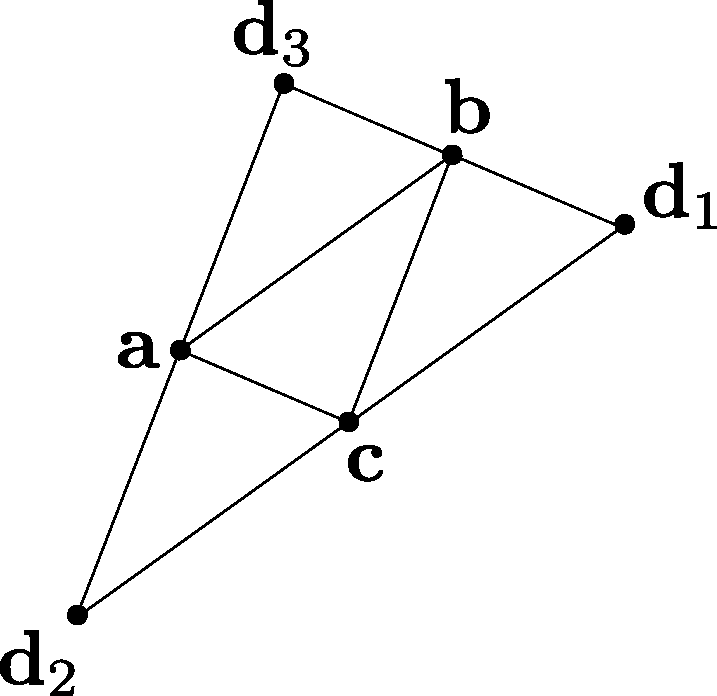
\includegraphics[width=1.5in]{figures/three_classes.pdf}
  \caption{The three equivalence classes: $A(\mathbf{a}, \mathbf{b},
  \mathbf{c}, \mathbf{d}_1), A(\mathbf{a}, \mathbf{b}, \mathbf{d}_2,
  \mathbf{c})$ and $A(\mathbf{a}, \mathbf{c}, \mathbf{d}_3,\mathbf{b})$.}
\label{FIG:3_classes}
\end{figure}

Let us mention an important point: if $a, b, c, d$ are not all distinct, the
equivalence classes contain less than $8$ proportions. This is natural,
because there are no longer $24$ different orderings of $a, b, c, d$. For
example if $a = c$ and $b = d$, then the equivalence class that is generated by
$A(a, b, c, d)$ is only made of $4$ proportions:
$$A(a, b, c, d) \eqdef A(a, b, a, b) \iff A(a, a, b, b) \iff A(b, b, a, a) \iff
(b, a, b, a).$$

Although these notions may seem shallow at first sight, they will actually turn
out to be paramount to grasp the geometrical view of Boolean proportions that
we now address.

\subsection{The Boolean and arithmetic proportions as parallelograms}

What we know so far is that the arithmetic proportion in $\mathbb{R}^m$
involves the four vertices of a parallelogram. As for the Boolean proportion,
we know from Definition \ref{DEF:analogy_for_vectors} that four Boolean vectors
$\mathbf{a}, \mathbf{b}, \mathbf{c}, \mathbf{d}$ are in proportion if each
component build up a valid proportion, i.e. that each of the $(a_i, b_i, c_i,
d_i)$ follow one of the $6$ valid patterns of Table
\ref{TAB:six_valid_patterns} on page \pageref{TAB:six_valid_patterns}.
\begin{testexample}
For example in $\mathbb{B}^2$, the four vectors $\mathbf{a} = (0, 0),~
  \mathbf{b} = (1, 0),~ \mathbf{c} = (0, 1)$ and $\mathbf{d} = (1, 1)$ are in
  proportion because the two component-wise proportions $a_1 : b_1 :: c_1 :
  d_1$ and $a_2 : b_2 :: c_2:d_2$ are valid: we have $0: 1 :: 0: 1$ and
  $0:0::1:1$.

  The four vectors $\mathbf{a} = (0, 0),~ \mathbf{b} = (1, 0),~ \mathbf{c} =
  (0, 1)$ and $\mathbf{d} = (1, 0)$ are \textbf{not} in proportion because $a_2
  : b_2 :: c_2 : d_2$ is not a valid pattern.
\end{testexample}

We have also seen that in $\mathbb{B}$, the Boolean
proportion and the arithmetic proportion are equivalent. This is also naturally
the case in $\mathbb{B}^m$! This means that a proportion in $\mathbb{B}^m$ can
also be represented as a (potentially \textit{flat}) parallelogram. By
\textit{flat} parallelogram we mean that the four vertices are not all
distinct: this will all become clear by looking at the two following
illustrations, in $\mathbb{B}^2$ and in $\mathbb{B}^3$.

\paragraph{The $36$ proportions of $\mathbb{B}^2$\\}

Figure \ref{FIG:proportions_in_B2} illustrates the proportions that
one can build in $\mathbb{B}^2$:
\begin{itemize}
  \item The proportion $\mathbf{a}: \mathbf{b} :: \mathbf{c} : \mathbf{d}$ and
    its 7 other equivalent forms, making up the parallelogram
    $\mathbf{a}\mathbf{b}\mathbf{c}\mathbf{d}$ (remember that when all elements
    are distinct, the equivalence class represented by $A(\mathbf{a},
    \mathbf{b}, \mathbf{c}, \mathbf{d})$ is composed of $8$ elements).
  \item The proportions that we can build using any pair of vertices, for
    example $\mathbf{a} : \mathbf{d} :: \mathbf{a} : \mathbf{d}$. Each of these
    proportions has $3$ other equivalent forms: in this case $\mathbf{a} :
    \mathbf{a} :: \mathbf{d} : \mathbf{d}$, $\mathbf{d} : \mathbf{a} ::
    \mathbf{d} : \mathbf{a}$ and $\mathbf{d} : \mathbf{d} :: \mathbf{a} :
    \mathbf{a}$. As there are $\binom{4}{2} = 6$ pairs of vertices in
    $\mathbb{B}^2$, there are exactly $6 \times 4$ proportions of this kind,
    all of which are flat\footnote{The \textit{flat} proportion are those that make
    up flat parallelograms. This naming convention is actually fortunate,
    because these proportions are in practice absolutely useless, as it will
    soon become clear in the next section.}.
  \item The $4$ proportions involving each vertex independently, for example
    $\mathbf{b}:\mathbf{b}::\mathbf{b}:\mathbf{b}$. These proportions are also
    flat, naturally.
\end{itemize}

\begin{figure}[!h]
\centering
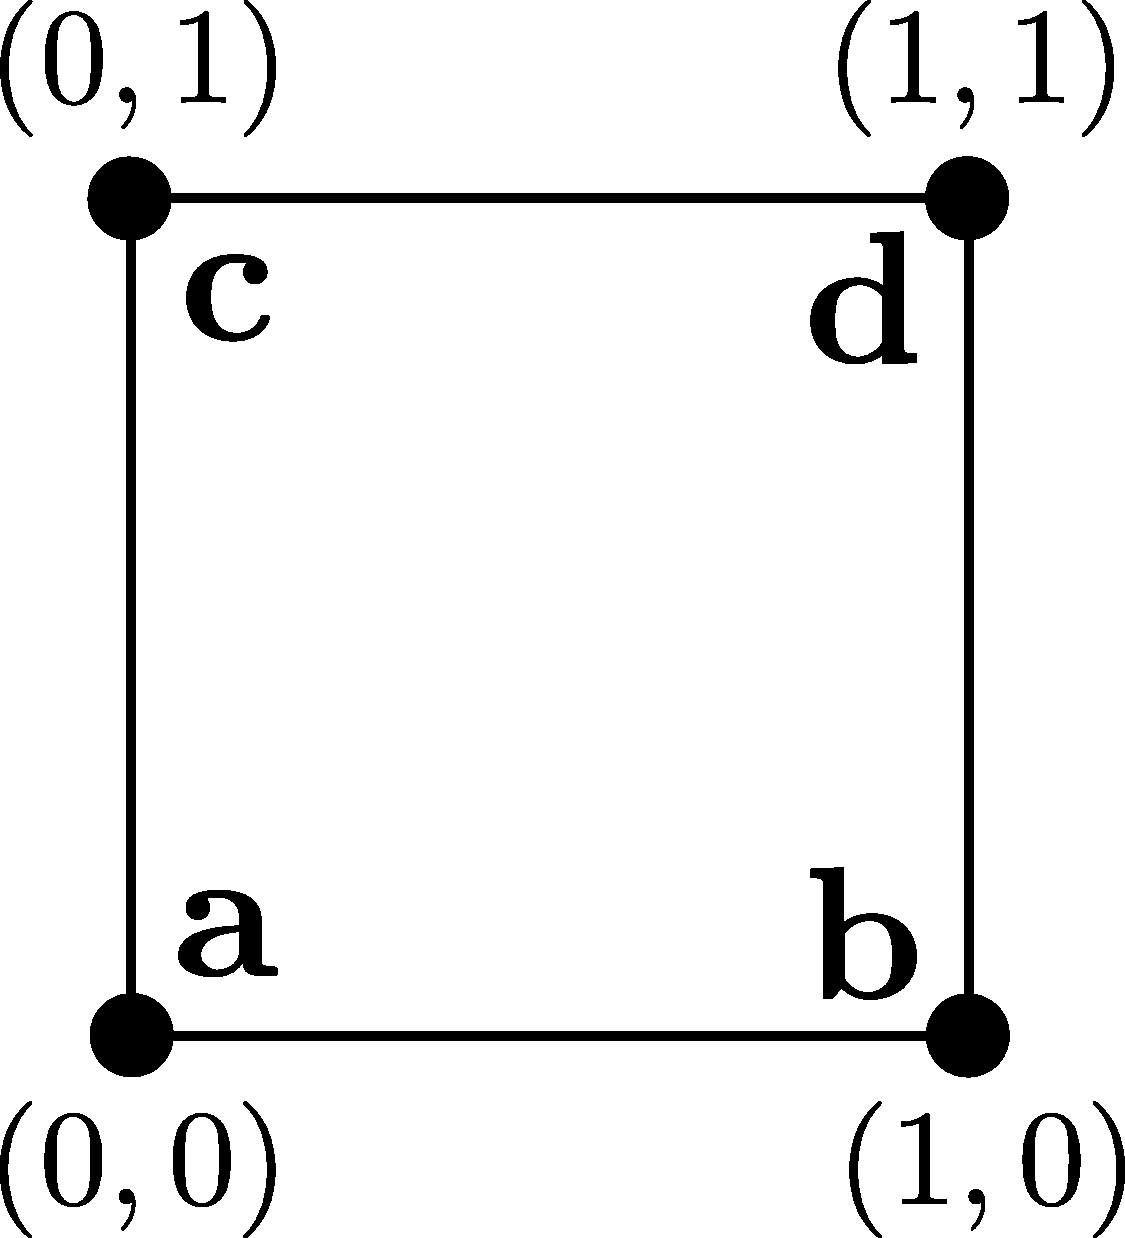
\includegraphics[width=1.5in]{figures/proportions_in_B2.pdf}
  \caption{The $36$ proportions in $\mathbb{B}^2$.}
\label{FIG:proportions_in_B2}
\end{figure}

All in all, this makes up to $36 = 8 + 6 \times 4 + 4$ proportions: $8$
proportions from the parallelogram $\mathbf{a}\mathbf{b}\mathbf{c}\mathbf{d}$,
$6 \times 4$ proportions from the pairs of vertices, and $4$ proportions from the
$4$ vertices. In fact, this number of $36$ proportions could have been derived
directly by remembering that in $\mathbb{B}^2$ the proportions are defined in a
component-wise fashion, and that there are exactly $6$ valid patterns of
proportions in $\mathbb{B}$: as a proportion in $\mathbb{B}^2$ is the
concatenation of two proportions in $\mathbb{B}$, the number of valid
proportions in $\mathbb{B}^2$ necessarily is $6 \times 6 = 36$.

Let us also note though that only $1 + 6 + 4 = 11$ of them can be considered
\textit{unique} (up to equivalence) and only one is non-flat. In the next
section, we will further investigate the number of unique proportions that can
be built in $\mathbb{B}^m$.

\paragraph{The proportions of $\mathbb{B}^3$\\}

Going a dimension further can still be insightful. Figure \ref{FIG:cubes_in_B3}
illustrates the 12 non-flat proportions that exist in $\mathbb{B}^3$. These
proportions are the parallelograms making up the 6 faces of the $3$-cube, and
six other \textit{diagonal} parallelograms passing through the center of the
cube.  The flat proportions are not shown for the sake of clarity.

\begin{figure}[!h]
\centering
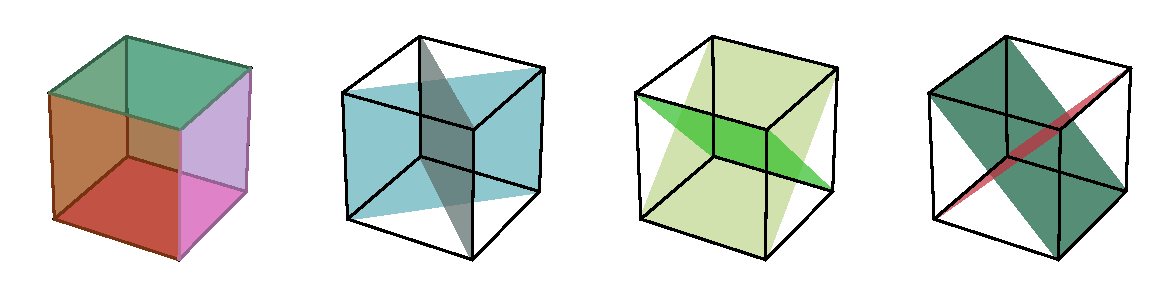
\includegraphics[width=\linewidth]{figures/cubes_in_B3.pdf}
  \caption{The $12$ \textit{non-flat} parallelograms in $\mathbb{B}^3$: the
  six faces of the cube, and $3 \times 2$ \textit{diagonal} parallelograms,
  e.g. $(000) : (010) :: (101) : (111)$.}
\label{FIG:cubes_in_B3}
\end{figure}

Let us finally note the following remarkable property, which will be useful to
us much later in Chapter \ref{CHAP:analogy_preserving_functions}:

\begin{property}
  \label{PROPER:hamming_distance_boolean_proportion}
  Let $\mathbf{a}, \mathbf{b},\mathbf{c}, \mathbf{d}$ in $\mathbb{B}^m$, and
  let $H(\mathbf{x}, \mathbf{x'})$ be the Hamming distance between $\mathbf{x}$
  and $\mathbf{x'}$, i.e. the number of components we need to flip to transform
  $\mathbf{x}$ into $\mathbf{x'}$ (or the reverse).\\
  If $\mathbf{a} : \mathbf{b}
  :: \mathbf{c} : \mathbf{d}$, then these three equalities hold:

  $$
  \begin{cases}
    H(\mathbf{a}, \mathbf{b}) = H(\mathbf{c}, \mathbf{d})\\
    H(\mathbf{a}, \mathbf{c}) = H(\mathbf{b}, \mathbf{d})\\
    H(\mathbf{a}, \mathbf{d}) = H(\mathbf{b}, \mathbf{c}).
  \end{cases}
  $$
\end{property}

We can easily verify this property in $\mathbb{B}$ from Table
\ref{TAB:six_valid_patterns}, and the general case in $\mathbb{B}^m$ immediately
follows from Definition \ref{DEF:analogy_for_vectors}. Sadly, Property
\ref{PROPER:hamming_distance_boolean_proportion} only offers a necessary
condition for a proportion to hold, and not a sufficient one: indeed taking $a
= d = 1$ and $b = c =0$ in $\mathbb{B}$, the three equalities are clearly
respected but $1:0::0:1$ is not a valid proportion. The first two
properties $H(\mathbf{a}, \mathbf{b}) = H(\mathbf{c}, \mathbf{d})$ and
$H(\mathbf{a}, \mathbf{c}) = H(\mathbf{b}, \mathbf{d})$ are classical
properties for parallelograms, but interestingly the third one $H(\mathbf{a},
\mathbf{d}) = H(\mathbf{b}, \mathbf{c})$ is only true for rectangles. In fact,
the parallelograms that we can build in $\mathbb{B}^m$ are \textbf{always}
rectangles.\\


This closes this discussion on the geometric interpretation of Boolean
proportions. In the next section we will apply the previously described notions
to a task of classification, which will help us to introduce new concepts, and
also to make a smooth transition towards the next chapter.

\section{Analogical inference principle and equation solving}
\label{SEC:machine_learning_with_boolean_proportions}

The goal of this last section is to introduce two other fundamental notions
that will be used in our investigations: the \textbf{analogical inference
principle}, and the process of \textbf{analogical equation solving}. Once
combined, these two concepts allow us to perform inference, and to apply
analogical reasoning to machine learning tasks such as classification.

We will here consider a toy classification problem in a Boolean setting, which
will help us introduce these two fundamental notions. This toy problem will
also serve as an introduction to the next chapter, where we will study the
theoretical properties of analogical classifiers. Because of the nature of the
problem, this section will be a mix of particular and general considerations.

\paragraph{Problem setting\\}

We now have enough background on Boolean proportions to start doing some
machine learning. Here is our problem. We consider the set $\mathbb{B}^m$ and
its $2^m$ elements. For various $\mathbf{x} \in \mathbb{B}^m$, we know the
value of $f(\mathbf{x})$, where $f$ is a function from $\mathbb{B}^m$ to
$\mathbb{B}$.  The value $f(\mathbf{x})$ is called the \textbf{class} of
$\mathbf{x}$, or its \textbf{label}. The set $S \subsetneq \mathbb{B}^m$ of
elements for which $f(\mathbf{x})$ is known is called the \textbf{training
set}. For any element $\mathbf{x} \notin S$, $f(\mathbf{x})$ is unknown and our
goal is to guess it: this is a binary \textbf{classification problem}.

Suppose we're in $\mathbb{B}^3$ and consider Figure
\ref{FIG:classification_problem}.
\begin{figure}[!h]
\centering
  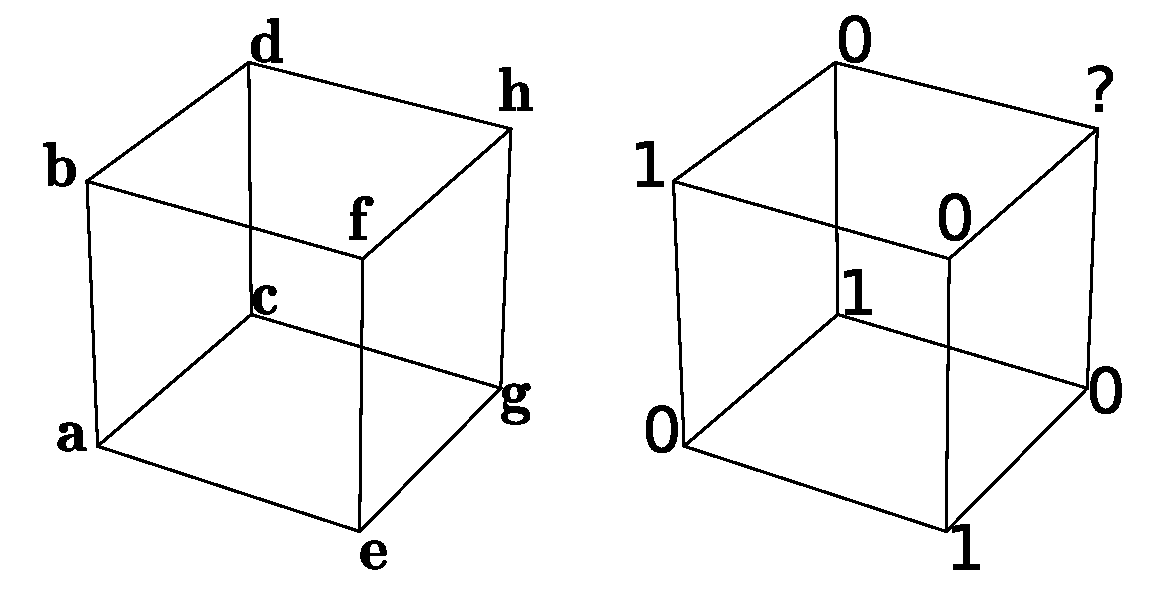
\includegraphics[width=3in]{figures/classification_problem.pdf}
  \caption{A classification problem in $\mathbb{B}^3$. Labels $f(\mathbf{x})$
  are on the right cube.}
\label{FIG:classification_problem}
\end{figure}
We know the values of $f(\mathbf{x})$ for
every single element $\mathbf{x}$ but $\mathbf{h}$, so $S = \{ \mathbf{a}, \mathbf{b},
\mathbf{c}, \mathbf{d}, \mathbf{e}, \mathbf{f}, \mathbf{g}\}$. There are
numerous methods at hand to go guess the value of $f(\mathbf{h})$. One of the
most famous one is the nearest neighbors heuristic, which would lead us to
consider that the label of $\mathbf{h}$ is the same as  that of its
\textit{neighbors}, i.e. the elements that are close to $\mathbf{h}$ with
respect to a given distance function. Using the Hamming distance, we would
assign to $\mathbf{h}$ the label $0$, because the $3$ closest neighbors of
$\mathbf{h}$, namely $\mathbf{d}, \mathbf{f}, \mathbf{g}$, are all labeled with
$0$.

\paragraph{The analogical inference principle\\}

Our point is here to describe the process of analogical classification, so we
will forget the nearest neighbor heuristic and we will instead make use of the
so-called \textbf{analogical inference principle}, which states that if four
elements $\mathbf{x}, \mathbf{y}, \mathbf{z}, \mathbf{t}$ are in proportion,
then their labels should also be in proportion:
$$
\infer[\text{Analogical inference principle}]{\mathbf{x} : \mathbf{y} ::
\mathbf{z} : \mathbf{t}}{f(\mathbf{x}) : f(\mathbf{y}) :: f(\mathbf{z}) :
f(\mathbf{t})}
$$

This is obviously an unsound principle, in that the conclusion does not
logically follows from the premise. But as we will see in this document, it can
still be useful.

The key point here is that if the value of $f(\mathbf{t})$ is unknown, it can
be \textbf{recovered} from the values of $f(\mathbf{x}), f(\mathbf{y}),
f(\mathbf{z})$ by the process of \textbf{analogical equation solving} that we
explain now.

We here want to guess the
value of $f(\mathbf{h})$. The analogical inference principle leads us to look
for all 3-tuples $(\mathbf{x}, \mathbf{y}, \mathbf{z}) \in S^3$ such that
$\mathbf{x}:\mathbf{y}::\mathbf{z}:\mathbf{h}$ holds.  The principle then states that
for all of these $3$-tuples, we should have
$f(\mathbf{x}):f(\mathbf{y})::f(\mathbf{z}):f(\mathbf{h})$.
Figure \ref{FIG:cubes_in_B3} tells us that there are 6 (non-flat)
parallelograms involving $\mathbf{h}$ as a vertex. The six unique corresponding
proportions are:

\begin{enumerate}
  \item $\mathbf{a} : \mathbf{b} :: \mathbf{g} : \mathbf{h}$
  \item $\mathbf{a} : \mathbf{d} :: \mathbf{e} : \mathbf{h}$
  \item $\mathbf{a} : \mathbf{c} :: \mathbf{f} : \mathbf{h}$
  \item $\mathbf{b} : \mathbf{d} :: \mathbf{f} : \mathbf{h}$
  \item $\mathbf{e} : \mathbf{f} :: \mathbf{g} : \mathbf{h}$
  \item $\mathbf{c} : \mathbf{g} :: \mathbf{d} : \mathbf{h}$.
\end{enumerate}

Applying the analogical inference principle to the first proportion $\mathbf{a}
: \mathbf{b} :: \mathbf{g} : \mathbf{h}$ leads to $f(\mathbf{a}) :
f(\mathbf{b}) :: f(\mathbf{g}) : f(\mathbf{h})$, which is equivalent to:
$$0:1::0:f(\mathbf{h}).$$ By referring to Table \ref{TAB:six_valid_patterns} on
page \pageref{TAB:six_valid_patterns}, we
notice that $f(\mathbf{h})$ should be equal to $1$ for the proportion
$f(\mathbf{a}) : f(\mathbf{b}) :: f(\mathbf{g}) : f(\mathbf{h})$ to be a valid
one, because $0:1::0:1$. So we keep $1$ in the back of our head as a possible
candidate for $f(\mathbf{h})$: we say that $1$ is a \textbf{candidate
solution} for $f(\mathbf{h})$.  What we have just done is the \textbf{solving
of an analogical equation}.

\paragraph{Analogical equation solving in general\\}

Generally speaking, an analogical equation is a proportion $a:b::c:x$ in a
context where $x$ is unknown. Determining the value of $x$ is then called the
\textit{solving} of this equation. Depending on the nature and values of $a, b,
c$, there may or may not exist a solution, and it might not be unique.

In fact, we have all been solving analogical equations since our childhood,
because in the case of the geometric proportion it reduces to the well known
rule of three: $\frac{5}{2} = \frac{10}{x} \implies x = \frac{2 \times 10}{5} =
4$, and generally $a:b::c:x \implies x = \frac{b \times c}{a}$ ($a \neq 0$).
The solution of the arithmetic proportion $a - b = c -x$ is also extremely
simple and is given by $x = c - a + b$.

In a Boolean setting, an equation is solvable for 6 patterns of $a, b, c$ (the
6 patterns of Table \ref{TAB:six_valid_patterns}, naturally):
\begin{proposition}
  \label{PROPOS:equation_solving}
  Let $a, b, c$ in $\mathbb{B}$. The analogical equation
  $a :b::c:x$
  is solvable if and only if $a = b$ or $a = c$. The solution denoted
  $\emph{sol}(a, b, c)$ is always unique and is given by:
  $$
  \begin{cases}
    \emph{sol}(a, b, c) \eqdef c \emph{~~ if } a = b,\\
    \emph{sol}(a, b, c) \eqdef b \emph{~~ if } a = c,
  \end{cases}
  $$
  or more generally:
  $$\emph{sol}(a, b, c) \eqdef c - a + b,$$
  because the Boolean proportion is a particular case of the arithmetic
  proportion. The values of $\emph{sol}(a, b, c)$ for all the Boolean $3$-tuples $(a,
  b, c)$ are given in Table \ref{TAB:solutions}.
\end{proposition}

\begin{table}[t]
  \centering
  \begin{tabular}[t]{cccc}
    \toprule
    $a$ & $b$ & $c$ & $\sol(a, b, c)$ \\
    \midrule
    0 & 0 & 0 & 0 \\
    1 & 1 & 1 & 1 \\
    0 & 0 & 1 & 1 \\
    1 & 1 & 0 & 0 \\
    0 & 1 & 0 & 1 \\
    1 & 0 & 1 & 0 \\
    1 & 0 & 0 &?\\
    0 & 1 & 1 &?\\
    \bottomrule
  \end{tabular}
  \caption{The solutions $\sol(a, b, c)$ for every Boolean $3$-tuple $(a, b,
  c)$. The question mark $?$ means that $\sol(a, b, c)$ is undefined. We can
  verify that $\sol(a, b, c) = c - a + b$ when the solution is defined.}
  \label{TAB:solutions}
\end{table}

\paragraph{Back to the estimation of $f(\mathbf{h})$\\}

Let's get back to the estimation of $f(\mathbf{h})$. Applying the analogical
inference principle to the second proportion $\mathbf{a} : \mathbf{d} ::
\mathbf{e} : \mathbf{h}$ leads $f(\mathbf{a)} : f(\mathbf{d}) :: f(\mathbf{e})
: f(\mathbf{h})$, and to the solving of $0:0::1:f(\mathbf{h})$. Here again, the
solution is $1$, just like the candidate of the first proportion.
The third proportion  $\mathbf{a} : \mathbf{c} :: \mathbf{f} : \mathbf{h}$
leads to the solving of $0:1::0:f(\mathbf{h})$, also claiming that $1$ is a good candidate.

And now the fourth proportion $\mathbf{b} : \mathbf{d} :: \mathbf{f} :
\mathbf{h}$, which leads to $1:0::0:f(\mathbf{h})$. \textbf{This equation is not
solvable}: neither $1:0::0:1$ nor $1:0::0:0$ are valid proportions. We can also
check this fact from Table \ref{TAB:solutions}. We thus
simply discard the proportion $\mathbf{b} : \mathbf{d} :: \mathbf{f} :
\mathbf{h}$ as a potential source of information about $f(\mathbf{h)}$, because
we are not in a position to apply the analogical inference principle. We can
easily verify that the fifth and sixth proportions also lead to non-solvable
equations.

All in all, we are left with three candidates coming from the first three
proportions, all of which are equal to $1$. Our guess will thus be that
$f(\mathbf{h})$ should be equal to $1$, so we will set the \textbf{estimation} of
$f(\mathbf{h})$ as $\hat{f}(\mathbf{h}) = 1$.
Notice that we have so far completely ignored  all the flat proportions,
i.e. proportions where the four elements are not all distinct.
This is because none of these proportions allow us to derive a solvable
equation. Considering for example $\mathbf{d} : \mathbf{h} :: \mathbf{d} :
\mathbf{h}$, we're led to the solving of $f(\mathbf{d}) : f(\mathbf{h}) ::
f(\mathbf{d}) : f(\mathbf{h})$, or equivalently of $0 : f(\mathbf{h}) :: 0 :
f(\mathbf{h})$. Both values $0$ and $1$ could lead to equally valid proportions
here, so there is simply no predictive power in the flat proportions. We have
also only considered unique proportions, up to equivalence. The first proportion
$\mathbf{a} : \mathbf{b} :: \mathbf{g} : \mathbf{h}$ for example is equivalent
to $\mathbf{a} : \mathbf{g} :: \mathbf{b} : \mathbf{h}$ (using central
permutation), which we could have
used instead. As any two equivalent proportions lead to the same solution for
their associated class equations, we usually choose to ignore all other equivalent
proportions, which allows to divide the number of equation solving processes by
a factor of $2$.

\paragraph{The analogical classification process: summary\\}

Here is a small outline of the classification process we have just followed,
that was entirely governed by the analogical inference principle. Our goal was
to guess the value of $f(\mathbf{h})$:

\begin{itemize}
  \item We first looked at all the $3$-tuples $(\mathbf{x}, \mathbf{y}, \mathbf{z}) \in
    \mathbf{B}^3$ such that:
    \begin{itemize}
      \item $f(\mathbf{x}), f(\mathbf{y})$ and $f(\mathbf{z})$ are known ;
      \item $\mathbf{x}:\mathbf{y}::\mathbf{z}:\mathbf{h}$ holds ;
      \item the \textbf{class equation} $f(\mathbf{x}) :f(\mathbf{y}) ::
        f(\mathbf{z}) :s$ is \textbf{solvable}. $s$ is called a
        \textbf{candidate solution}.
    \end{itemize}
    Each of the three candidate solutions $s_1, s_2, s_3$ agreed on the same prediction:
    $s_i = 1$ for all $i$.
  \item We thus estimated that $f(\mathbf{h})$ should indeed be equal to $1$.
\end{itemize}

\paragraph{Open questions\\}

This minimal example of analogical classification raises a few concerns, which
will be thoroughly addressed in the rest of this document:
\begin{enumerate}
  \item All of the three candidate solutions for $f(\mathbf{h})$ agreed on the
    same prediction: $1$. What if one of them predicted $0$? A first drastic
    option is to refuse to classify $\mathbf{h}$, on the basis that if the
    candidates cannot agree on their predictions, then we should not trust any
    of them. As it will become clear, in practice the candidates never really
    completely agree, even though sometimes a clear majority emerges. So this
    strategy would make the prediction impossible for most elements $\mathbf{x}
    \notin S$. A wiser option is to consider an aggregation of the candidate
    solutions: the most common one, for example. This is the option that has
    been taken on so far, as we will see in the next chapter.
  \item Here, by chance, the set of candidate solutions for $f(\mathbf{h})$ was
    not empty: we found three candidate solutions. What happens if we cannot
    find any candidate? This case arises when there are no 3-tuple
    $(\mathbf{x}, \mathbf{y}, \mathbf{z}) \in S^3$ such that $\mathbf{x} :
    \mathbf{y}::\mathbf{z}:\mathbf{h}$ holds and such that the associated equation
    $f(\mathbf{x}):f(\mathbf{y})::f(\mathbf{z}):f(\mathbf{h})$ is solvable. In
    the works of Stroppa and Yvon (\cite{StrYvoCNLL05}), such an $\mathbf{h}$
    cannot be classified. The notion of \textbf{analogical dissimilarity} as
    used in \cite{BayMicDelIJCAI07} will allow to bypass this issue. In the
    next chapter, we will detail these two versions of analogical learning, and
    one of the contributions of our work is to provide a unifying view of the
    two techniques.
  \item We have entirely relied on the analogical inference principle to
    classify $f(\mathbf{h})$. How \textit{safe} is this inference principle?
    Can we find some theoretical guarantees that could allow us to use it on a
    sound basis? In Chapter \ref{CHAP:analogy_preserving_functions}, we
    will provide a complete characterization of the Boolean functions $f$ that
    allow to derive sound conclusions.\\
\end{enumerate}

\noindent
Before moving further to the next section, let us  consider a seemingly trivial
question: how many proportions can we build in $\mathbb{B}^m$? As we will see,
this question will provide us with some further insight about the Boolean proportion.
This last discussion is, however, not as important as the previous ones and can
safely be ignored by the impatient reader.

\paragraph{How many proportions can we build in $\mathbb{B}^m$?\\}
\label{SEC:number_of_parallelograms_in_Bm}

Exactly $6^m$! And it is fairly easy to derive: there are $6$ proportions in
$\mathbb{B}$. As a proportion in $\mathbb{B}^2$ is the concatenation of any two
proportions in $\mathbb{B}$, there are exactly $6^2 = 36$ proportions in
$\mathbb{B}^2$, as seen in the previous section. Analogical proportions in
$\mathbb{B}^m$ are defined component-wise, i.e. they are the concatenation of
$m$ proportions in $\mathbb{B}$. Equivalently, a proportion in $\mathbb{B}^m$
is the concatenation of a proportion in $\mathbb{B}^{m - 1}$ and a proportion
in $\mathbb{B}$. By trivial induction, we can build $6^m$ proportions in
$\mathbb{B}^m$.

But let's now ask a more relevant and challenging question: \textbf{how many
\textit{useful} proportions can we build in $\mathbb{B}^m$?} By
\textit{useful}, we mean proportions that could be used for classification
purposes.  We have seen in this section that the only proportions
$\mathbf{a} : \mathbf{b} :: \mathbf{c} : \mathbf{d}$ that are useful for
classification purposes are those where all elements $\mathbf{a}, \mathbf{b},
\mathbf{c}, \mathbf{d}$ are distinct, i.e. the non-flat proportions. We thus
want to exclude from the $6^m$ proportions those that comply with one of the
following patterns:

\begin{itemize}
  \item $\mathbf{a}: \mathbf{a} :: \mathbf{a} : \mathbf{a}$ ;
  \item $\mathbf{a}: \mathbf{b} :: \mathbf{a} : \mathbf{b}$, and its three
    equivalent forms $\mathbf{a}: \mathbf{a} :: \mathbf{b} : \mathbf{b}$,~
    $\mathbf{b}: \mathbf{a} :: \mathbf{b} : \mathbf{a}$, and $\mathbf{b}:
    \mathbf{b} :: \mathbf{a} : \mathbf{a}$.
\end{itemize}

Now, let's count them.

\begin{itemize}
  \item Each of the $2^m$ vertices $\mathbf{a}$ will generate a proportion of the
    form $\mathbf{a}: \mathbf{a} :: \mathbf{a} : \mathbf{a}$, so there are
    exactly $2^m$ proportions of this kind.
  \item Every pair $(\mathbf{a}, \mathbf{b})$ of vertices will generate four
    proportions:
    \begin{itemize}
      \item $\mathbf{a}: \mathbf{b} :: \mathbf{a} : \mathbf{b}$ ;
      \item $\mathbf{a}: \mathbf{a} :: \mathbf{b} : \mathbf{b}$ ;
      \item $\mathbf{b}: \mathbf{a} :: \mathbf{b} : \mathbf{a}$ ;
      \item $\mathbf{b}: \mathbf{b} :: \mathbf{a} : \mathbf{a}$.
    \end{itemize}
    There are $\binom{2^m}{2}$ distinct pairs of vertices, so in total this
    makes $4\cdot \binom{2^m}{2}$ proportions of the form $\mathbf{a}: \mathbf{b} ::
    \mathbf{a} : \mathbf{b}$ with its equivalent forms.
\end{itemize}

We are then left with the number of $6^m - 2^m - 4\cdot\binom{2^m}{2}$ useful
proportions. We know that for each of these proportions, all elements
$\mathbf{a}, \mathbf{b}, \mathbf{c}, \mathbf{d}$  are distinct. For each of
them, there are thus 7 other equivalent forms, which reduces the number of
useful and unique (up to equivalence) proportions to:
$$P_m = \frac{1}{8} \left[6^m - 2^m - 4\cdot\binom{2^m}{2} \right].$$
Table \ref{TAB:n_params_in_cube} gives the values of $P_m$ for the first $10$
values of $m$.
\begin{table}[h!]
\centering
  \begin{tabular}{ l  l }
\toprule
 $m$ & $P_m$\\
\midrule
    1	&	0\\
    2 &	1\\
    3	&	12\\
    4	&	100\\
    5 &	720\\
    6 &	4816\\
    7 &	30912\\
    8 &	193600\\
    9 & 1194240\\
    10 & 7296256\\
\bottomrule
\end{tabular}
\caption{Number of unique non-flat proportions in an $m$-dimensional cube.}
\label{TAB:n_params_in_cube}
\end{table}
Naturally, $P_2$ and $P_3$ are in accordance with the empirical  results from
Figures \ref{FIG:proportions_in_B2} and \ref{FIG:cubes_in_B3}. The fact that
$P_1 = 0$ means that no inference can be done with analogical proportion in
$\mathbb{B}$, which is perfectly normal: in $\mathbb{B}$, all proportions are
flat (i.e. the pattern is always $a:b::a:b$ or $a:a::b:b$).

In fact, it turns out that this sequence of numbers $0, 1, 12, 100\dots$ is
already known as the A016283 sequence from the OEIS\footnote{The On-line
Encyclopedia of Integer Sequences (\url{http://oeis.org/A016283}).}.
This sequence actually describes \textit{the number of rectangles that can be
formed from the vertices of an $m$-dimensional cube}, which is exactly
equivalent to the number of \textit{useful} proportions that we wanted to
compute. The formula given by the OEIS is:
$$P_m = \frac{6^m}{8} - 4^{m - 1} + 2^{m - 3},$$
and using the fact that $\binom{n}{k} = \frac{n}{k}\binom{n - 1}{k - 1}$, it
can be shown that the two formulas $\frac{1}{8} \left[6^m - 2^m -
4\cdot\binom{2^m}{2} \right]$ and $\frac{6^m}{8} - 4^{m - 1} + 2^{m- 3}$ are,
fortunately, equivalent. It would be interesting to find out how the OEIS
formula was derived, but in all fairness we have no idea of the process that
was used.

\section*{Conclusion}

In this chapter, we have given the necessary background on formal analogical
proportions, mostly focusing on Boolean proportions. We have seen that an
analogical proportion $A$ is a quaternary relation following three simple
axioms that were already known in Aristotle times.

In the first section, we formally defined various analogical proportions in different settings,
starting from the most general definitions for semigroups and groups, until we
reached the Boolean proportion. We also presented an extension of the Boolean
proportion to multiple-valued logics, which we will use much later in Chapter
\ref{CHAP:analogical_recommendation}.

In the second section, we extended our knowledge and understanding of the Boolean
proportion. We illustrated the close bonds that exist between the Boolean
proportion and the arithmetic proportion, and we showed that both can be seen
as a relation between the four vertices of a parallelogram in $\mathbb{B}^m$ or
in $\mathbb{R}^m$.

The third section was devoted to the description of the analogical inference
principle and of the analogical equation solving process. By solving an
analogical equation, we are able to infer some information about any of the
four elements at play in an analogy, provided that the three others are known.
This process can be seen as a simple generalization of the rule of three that
we have been using since childhood: $\frac{4}{2} = \frac{6}{x} \implies x =
3$. Using this powerful tool and applying the analogical inference principle,
we were able to go trough a simple classification problem in a Boolean setting.

The aim of these first two chapters was to provide an overview of past works in
analogical reasoning, and to provide the necessary background to understand the
contributions made in this thesis. In the next chapter, we will describe our
contributions to the task of analogical classification.
